\chapter{DELAY-INSENSITIVE MULTI-OBJECT MULTI-CAMERA TRACKING}

\section{Introduction}
Autonomous robotic weeding systems in precision farming have demonstrated their full potential to alleviate the current dependency on agrochemicals such as herbicides and pesticides, thus reducing environmental pollution and improving sustainability. 
However, most previous works require fast and constant-time weed detection systems to achieve real-time treatment, which forecloses the implementation of more capable but time-consuming algorithms, e.g. learning-based weed detection methods. 
To overcome such difficulty, a non-overlapping multi-camera system is applied to provide flexibility for the weed control system in dealing with the indeterminate classification delays.
Given the mostly static environment and rigidly connected but unsynchronized cameras, the multi-object multi-camera 3D tracking problem can be solved by formulating an intra-camera metric \acrshort{vslam} system, an inter-camera object tracking module, and a delay-insensitive object manager, where high-level objects, e.g. weeds or plants, can be geometrically modeled and tracked within and across cameras.
Considering the limited computational power of the onboard robotic platform and the unstructured agricultural environments, the two systems need to be deliberately designed for real-time reliable performance:
\begin{enumerate}
	\item For an embedded system, it is unrealistic to feed images from multiple cameras into a time-consuming weed/plant classifier at each iteration (10$fps$), especially when the one-image-per-iteration solution has already overwhelmed the onboard GPU. 
The limited access of object detection makes the efficient inter-camera sparse-to-sparse object association vanished. 
Instead, a sparse-to-dense inter-camera tracking algorithm with constrained search needs to be deliberately designed for real-time object localization. 
	\item To facilitate an efficient inter-camera object tracking, either the local image patch (direct) or the nearby features (indirect) can be extracted as object representation for tracking. 
However, either of them has faced certain levels of difficulties. 
For indirect approaches, the state-of-the-art features are more-or-less prohibited for this application. 
The fast binary features, e.g. ORB, are tested to be less repeatable and discriminative in small-scale agricultural environments, where the survived keypoints are usually too sparse to well-represent an object. 
The real-value features, e.g. SIFT, can be reliably tracked in this type of environment but have already been precluded by the overloaded computational power. 
For direct solutions, the inter-camera appearance change of the object template needs to be compensated for reliable tracking. 
	\item Unlike the pure plane ground in the city scene, the field of agriculture is typically modeled as 2.5D environments, where the depth variation is attributed to grown-up valuable plants.
Correspondingly, the conventional 2D template matching is considered to be insufficient, where a 3D-2D template tracking pipeline is in need.
\end{enumerate}

In this chapter, we concentrate on four key developments towards the above-mentioned problems: 
\begin{enumerate}
	\item \textbf{Intra-Camera Tracking} A monocular-sonar \acrshort{vo} system that simultaneously estimates metric camera trajectory and field ground reconstruction through bundle adjustment with depth regulation.
	\item \textbf{Inter-Camera Tracking} An illumination-robust multi-object 3D-2D tracking algorithm that helps to retrace detected objects across cameras. 
	\item \textbf{Delay-Insensitive Object Management} An object initializer and updater that receives delayed object detection results from the classifier, reconstruct, and propagate the 3D positions of detected objects across cameras.
	\item \textbf{Integrated Weed Control System} An integrated weed control system that combines state-of-the-art weed/plant classifier, delay-insensitive multi-object multi-camera tracker, and predictive controller for high-precision weed removal.
\end{enumerate}

\section{Background}
\noindent \textbf{Intra-Camera Tracking}
The intra-camera tracking is essentially a \acrshort{vslam}/\acrshort{vo} system, which can be generally divided into two categories: indirect and direct methods. 
Indirect methods, \cite{klein2007parallel} \cite{mur2017orb}, pre-process acquired an image to extract a certain type of features, which is utilized to recover the camera pose and scene structure by minimizing geometric error. 
Unlike indirect approaches relying on features, direct methods directly use intensities of the image to estimate camera motion and scene structure rather than features. 
For direct dense mapping, \cite{stuhmer2010real} \cite{newcombe2011dtam} \cite{pizzoli2014remode}, the photometric error with spacial geometry prior formulations are developed to reconstruct a dense depth map and corresponding camera motion accurately. 
However, the real-time performance of such methods can only be guaranteed by introducing modern, powerful GPU due to their intensive computational load. 
To ease the computational demand, the semi-dense methods, \cite{engel2013semi} \cite{engel2014lsd}, reconstruct the inverse depth map through pixel-wise small-baseline stereo comparisons instead of joint optimization, enabling real-time CPU implementation. 
More recently, a direct sparse formulation \cite{engel2018direct} was proposed to jointly optimize motion and structure by omitting the smoothness prior, which makes real-time performance feasible. 
In recent years, direct approaches have attracted more attention due to their higher accuracy and robustness in both tracking and reconstruction, compared with indirect methods. 
The main advantage of the direct formulation is that the scene points are not required to be self-recognizable, thus allowing for more complete usage of information in an image. 
As a result, such characters of direct formulation makes it quite suitable for our intra-camera tracking application. 

\noindent \textbf{Inter-Camera Tracking} 
Weed tracking across non-overlapping cameras, named inter-camera tracking, mainly concentrates on object occlusion, cross-camera appearance ambiguities, and illumination changes. 
However, our proposed system implements fixed-viewpoint down-looking cameras with an artificial lighting system, so that only the illumination difference between cameras needs to be carefully treated. 
In recent years, a number of illumination-robust \acrshort{vo} and \acrshort{vslam} systems have been proposed, implementing various models or descriptors to alleviate the adverse effect of external lighting changes, to achieve robust tracking across cameras. 
To gain robustness against the global illumination changes, either the median value of pixel residuals \cite{meilland2011real} \cite{gonccalves2011real} \cite{bloesch2015robust} \cite{greene2016multi} or an affine brightness transfer function \cite{klose2013efficient} \cite{engel2015large} is estimated to compensate for the induced adverse effect in the optimization. 
For local lighting changes, \cite{dai2017bundlefusion} proposes to use image gradients, rather than pixel intensities, to formulate the direct energy function, thus gaining local lighting invariance. \cite{crivellaro2014robust} relies on the dense computation of a deliberately designed local descriptor to obtain a clear global minimum in energy function while preserving convergence basin by convolving with a low-pass filter. 
The methods based on the census transform \cite{alismail2016direct} use a binary descriptor to achieve local illumination invariance during the motion estimation. 

\section{Field Robot, Sensor Setup, and Datasets}

\begin{figure}[t]
	\centering
	\includegraphics[width=1.0\textwidth]{figures/agrirobotics/bonirob.pdf}
	\caption[Overview of Weed Control System]{\textbf{Overview of Weed Control System.} \textbf{Left}: The robotic platform Flourish BoniRob with our proposed weed control unit mounted at the bottom. \textbf{Right-Top}: A CAD view of the unit, including the actuators and sensors. \textbf{Right-Bottom}: The pictures of the selective sprayer and the mechanical stamping tool.
	\label{fig:argirobotics_bonirob}}
\end{figure}

\noindent \textbf{Field Robot} 
The BoniRob in \ref{fig:argirobotics_bonirob} is a multi-propose field robot designed by BOSCH DeepField Robotics, which provides an application bay to install various tools for specific tasks. 
In recent years, a variety of agriculture applications have been successfully developed and validated using this robot, such as selective spraying, mechanical weed control, as well as plant and soil monitoring.
In the Flourish Project, our proposed weed control system is mounted on a BoniRob, operating in various real field conditions to evaluate our proposed method.

\noindent \textbf{Sensor Setup} 
As the "eyes" of BoniRob, three ground-facing global shutter cameras (JAI AD-130 GE) with an 8$mm$ fix length lens (Fujinon TF15-DA-8) are mounted on our weed control unit. T
he distances to the ground is approximately 800$mm$, and the \acrlong{fov} (\acrshort{fov}) of each camera can reach up to 240${mm}$ x 310${mm}$. 
To protect the camera setup and the perception system from natural light sources, the weed control unit is covered by 3$mm$ acetal copolymer sheets, and artificial lights are mounted to control the illumination. 
As in most state-of-the-art weed detection algorithms, we use the \acrlong{ndvi} (\acrshort{ndvi}) \cite{lottes2016effective}, which utilizes both color (RGB) and the near-infrared (NIR) information. 
To do so, an RGB+NIR camera is used for the weed detection setup, whereas an RGB-only camera is used for the tracking setup since the additional NIR information comes typically at a high cost and is not required for the tracking part. 
Besides cameras, three narrow-beam sonars (SRF235 Ultrasonic Range Finder) are mounted next to each camera to help recover the absolute scale of the monocular \acrshort{vslam} estimates. 
The accuracy of the range measurement of these sonars is around 10$mm$.

\noindent \textbf{Dataset} We mainly evaluate our proposed system on sugar beet fields in Renningen (Germany), Ancona (Italy), and Zurich (Switzerland) in \ref{tbl:argirobotics_datasets}. In Renningen, we used faked weed targets (leaves) to quantitatively evaluate the performance of multi-camera tracking and inter-row weeding in different terrain conditions, speed, and various simulated classification delays. In Ancona and Zurich, the intra-row weeding is evaluated in a real field with typical weed species in \ref{fig:argirobotics_datasets}. The two datasets vary between 2-leaf and 4-leaf growth stages, which are the main stages of weeding for farmers. It should be noted that the sugar beets in Zurich dataset are at least four times larger compared to the ones in the Ancona dataset, which can be regarded as a harder dataset due to its increased environmental complexity.

\begin{table}[t]
\centering
\caption[Dataset Information]{Dataset Information} \label{tbl:argirobotics_datasets}
\begin{tabular}{rccc}
\hline
                  & \textbf{Renningen}      & \textbf{Ancona}                & \textbf{Zurich}                \\ \hline
$\#$ sequences     & 12             & 8                     & 5                     \\
$\#$ images        & 21,591               & 7,499                    & 4,218                      \\
approx. crop size & -              & 0.5 - 100 $cm^2$         & 100 - 900 $cm^2$         \\
approx. weed size & 0.5 - 3.0 $cm^2$  & 0.5 - 60.0 $cm^2$        & 0.5 - 60.0 $cm^2$        \\
driving speed     & 0.05 - 0.5 $m/s$  & 0.1 - 0.3 $m/s$          & 0.1 - 0.2 $m/s$          \\
classifier        & Vegetation Detection & \cite{lottes2017semi} & \cite{lottes2017semi} \\
runtime           & $\sim$8 $Hz$        & 3 - 5 $Hz$               & 3 - 5 $Hz$               \\ \hline
\end{tabular}
\end{table}

\begin{figure}[h] 
	\centering
	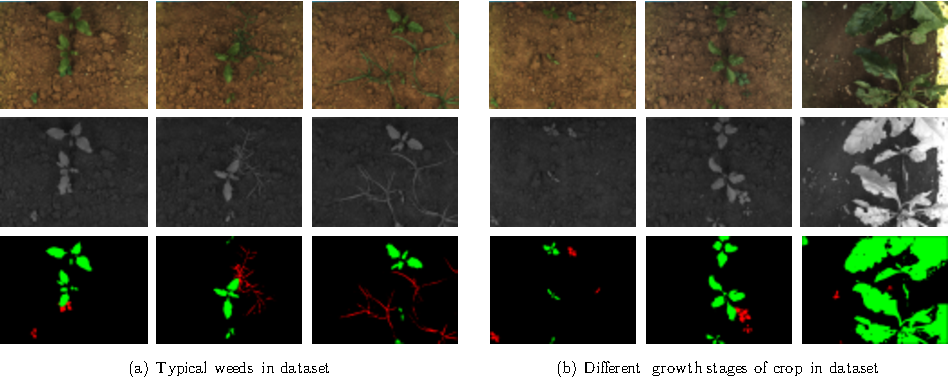
\includegraphics[width=\linewidth]{figures/agrirobotics/dataset.pdf}
	\caption[Typical Weeds and Growth Stages in Datasets]{ \textbf{Typical Weeds and Growth Stages in Datasets.} (a) Three typical weeds frequently observed in the datasets, where the RGB, NIR, and classification mask of pigweed (\textbf{Left}), crabgrass (\textbf{Middle}) and quackgrass (\textbf{Right}) are presented. (b) Three typical grow stages of crop in the datasets recorded in Ancona (\textbf{Left} and \textbf{Middle}) and Zurich (\textbf{Right}). 
	\label{fig:argirobotics_datasets}}
\end{figure} 

\section{Sensor Calibration}

\begin{figure}[t]
    \centering
    \includegraphics[width=\textwidth]{figures/agrirobotics/calibration.pdf}
    \caption[Multi-Camera and Camera-Sonar Calibration]{\textbf{Multi-Camera and Camera-Sonar Calibration.} \textbf{Left}: The calibration of non-overlapping cameras using overlapping calibration software by introducing an assistant camera in between. \textbf{Right}: The calibration of the camera and sonar height difference uses a marker field perpendicular to the central axes of the sensors.
	\label{fig:agrirobotics_calibration}}
\end{figure}

\noindent \textbf{Multi-Camera Calibration} 
To facilitate the high-precision estimation of the geometric properties of the weeds, all the intrinsic and extrinsic parameters of the non-overlapping camera system are calibrated. 
The intrinsic calibration for each camera is performed using standard OpenCV monocular calibration nodes \cite{bradski2000opencv}, where a pinhole camera model with radical tangential distortion parameters is estimated. 
The extrinsic calibration of our non-overlapping cameras is conducted using open-source overlapping camera calibration tool Kalibr \cite{furgale2013unified}, where an assistant camera is temporarily incorporated into the system to generate overlapping areas between the cameras, as shown in \ref{fig:agrirobotics_calibration} (a).

\textbf{Camera-Sonar Calibration} To compute the height difference between the camera and sonar, the marker field calibration \cite{siltanen2007automatic} between the camera and its corresponding sonar is conducted in \ref{fig:agrirobotics_calibration} (b). 
A set of artificial markers is attached on the flat ground surface inside the \acrshort{fov} of both camera and sonar, and the camera and sonar axis are placed perpendicular to the ground surface, thus allowing for the ground height estimation from both sensors. 
The measurements of heights from both sensors are processed and fed into a Kalman filter (KF), where the difference between two estimated heights is obtained as a calibration parameter. 

\section{Delay-Insensitive Multi-Object Multi-Camera Tracking} 
To provide reliable object tracking service across cameras regardless of classification delays, our proposed system can be generally divided into three components: intra-camera mapping and tracking, inter-camera tracking, and delay-insensitive multi-object management. 

\subsection{Intra-Camera Mapping and Tracking} 

The primary objective of our proposed intra-camera tracking algorithm is reconstruction and continuously tracking of the 3D positions of detected crops and/or weeds until retraced in the next camera or being treated.
Instead of tracking individual plants, we formulate our multi-object tracking as a metric \acrshort{vo} algorithm that performs camera tracking and ground object mapping by exploiting the domain knowledge that all tracked objects are stationary on the ground in \ref{fig:agrirobotics_intratracking}. 
Conventionally, multi-object tracking algorithms propose to receive classification results, extract the image template, then propagate its pose and tracking. 
In contrast, our proposed \acrshort{vo} approach recovers the 3D scene structure before obtaining object information, then formulating each template as a combination of trimmed image and inverse depth map for later tracking upon arrival of classification results. 
As a result, our proposed intra-camera tracking strategy guarantees a constant-time operation in spite of the change in the amount of tracked objects.

To improve the accuracy and robustness of weed estimates, the intra-camera tracking is developed based on direct structure and motion formulation, which does not use features at any stage of the algorithm.
Specifically, the intensity-based photometric error is selected since the appearance changes due to illumination variation is negligible under artificial lighting condition, thus satisfying brightness constancy assumption. 
To compute a meaningful metric estimation, the sonar measurements are merged into the photometric error minimization pipeline in \ref{eq:preliminaries_photometricerror} of \acrshort{vo} system as a depth regulation term:
\begin{equation} \label{eq:agrirobotics_metricvo}
\begin{split}
E_{kr}^{\mathcal{P}} &= \sum_{\mathbf{p}_r \in \mathit{S}_r^{\mathcal{P}}} w_{\mathbf{p}_r}^{\mathcal{P}} \Vert F_{k} ( \mathbf{p}_{kr}) - F_{r}(\mathbf{p}_r) \Vert_{\gamma} + \Vert D_r - z_{sonar}\Vert_{l1} \\
 \mathbf{p}_{kr} &=  \pi ( \mathbf{R}_{kr}\pi^{-1}(\mathbf{p}_r,D_{r}(\mathbf{p}_r) )+\mathbf{t}_{kr} )
\end{split} 
\end{equation} 

The algorithm consists of two major components: camera tracking and scene structure mapping in \ref{fig:agrirobotics_intratracking}, where the map is represented as inverse depth map as \cite{civera2008inverse}. 

\begin{figure}[t]
    \centering
    \includegraphics[width=\textwidth]{figures/agrirobotics/intra_tracking.pdf}
    \caption[Intra-Camera Mapping and Tracking]{\textbf{Intra-Camera Mapping and Tracking.} \textbf{Left}: The overview of our proposed intra-camera tracking and mapping algorithm. \textbf{Right}: Example reconstruction of the sugar beet using our proposed system. 
	\label{fig:agrirobotics_intratracking}}
\end{figure}

Many direct \acrshort{vo} algorithms prefer to use all pixels with significant gradient, named semi-dense methods. 
Incorporating as many pixels as possible into optimization is proven to improve the robustness and accuracy of pose estimates, however, also compromising the real-time performance. 
In this work, a sparse point selection strategy \cite{engel2018direct} is utilized to select well-distributed pixels spreading all over the image regions with sufficient gradients, which is proven to provide high-precision estimation in real-time. 
The 3D structure of the point candidates are initialized using the propagated inverse depth maps or pre-defined ground model through bilinear interpolation, then being tracked and optimized in camera tracking and environmental mapping phases.

\subsection{Inter-Camera Tracking}

\begin{figure}[t]
    \centering
    \includegraphics[width=0.8\textwidth]{figures/agrirobotics/inter_tracking.pdf}
    \caption[Inter-Camera Tracking]{\textbf{Inter-Camera Tracking.} The comparison of 2D-2D image matching and 3D-2D direct template matching methods for inter-camera tracking, where appearance variety induced by the viewpoint changes could make the conventional image matching completely fail.
	\label{fig:agrirobotics_intertracking}}
\end{figure}

The inter-camera tracking is designed to retrace the 2D positions of weeds using the information from images acquired from another camera, which forces us to take the illumination difference between cameras into consideration. 
To compensate for the appearance changes of weeds due to lighting variation and exposure difference, we can either plug global or local illumination-robust costs into our optimization framework described in \ref{eq:preliminaries_photometricerror}.
As stated in \cite{park2017illumination}, the global illumination-robust costs are capable of capturing whole image additive and/or multiplicative offsets, but failing to distinguish local lighting changes; the local ones, in contrast, can compensate both global and local illumination changes in the image, however, presenting significantly smaller convergence basin. 
For our weed control unit, both the global and regional illumination differences can be observed between images from different cameras due to the different lighting arrangements. 

Taking advantage that only the 2D positions of weeds in image space is of interest other than the estimation of camera poses, we extract the small frame template of each weed to perform local image alignment.
It combines the photometric error minimization with a global illumination affine model, thus alleviating the convergence issue by making local illumination consistency assumption.
For each object patch, the optimization problem can be expressed as:
\begin{equation} \label{eq:agrirobotics_affine}
\begin{split}
E_{c1,c2} &=  \sum_{\mathbf{p}_{c1} \in \mathcal{P}_{c1} } w_{\mathbf{p}_{c1}} \Vert F_{c1}(\mathbf{p}_{c1}) - \beta_{c1} - \frac{e^{\alpha_{c1}}}{e^{\alpha_{c2}}} F_k(\mathbf{p}_{c2,c1}) -\beta_{c2} \Vert_{\gamma} \\
 \mathbf{p}_{c2,c1} &=  \pi ( \mathbf{R}_{c2,c1}\pi^{-1}(\mathbf{p}_{c1},D_{c1}(\mathbf{p}_{c1}) )+\mathbf{t}_{c2,c1} )
\end{split} 
\end{equation}
where $\alpha_{c1,c2}$ and $\beta_{c1,c2}$ are global illumination affine model parameters, which are jointly optimized at each iteration. $\mathcal{P}_{c1}$ is a set of pixels within an extracted patch for a detected object. Combined with Huber norm, this affine model augmented method can work well in an environment without substantial local illumination changes.
 
Given the image $I_{c2}$ in the current camera and the weed frame template $\{ I_{c1}, D_{c1} \}$ from the previous camera, the objects are extracted and the object-wise relative pose $\mathbf{G}_{c1,c2} \in SE(3)$ is estimated by minimizing \ref{eq:agrirobotics_affine}. 
Then, the weed center and its template boundary are transformed into the current frame using the pose estimate, which is used to generate a new template for intra-camera tracking. 
It should be noted that the retrieval of the weed objects is achieved by using 3D-2D direct template-based matching instead of using conventional 2D-2D image correspondence since the change of viewpoint could induce significant changes of appearance of objects especially for the ones with high depth variance as shown in \ref{fig:agrirobotics_intertracking}.

\subsection{Delay-Insensitive Object Management}

To initialize the items in the object updater with the unpredictable delays, a time-stamp indexed frame buffer is preserved in the memory to ease the later searching and the pose propagation. 
Each frame in the buffer, indexed by the image capture time, contains the received gray-scale image, the estimated camera pose from the \acrshort{vo}, and the recovered inverse depth map. 
When a classification result arrives at the object initialization layer, the corresponding frame is extracted from the buffer given its time-stamp. 
The templates of the detected plants, consisting of a grey-scale image and inverse depth map, are extracted with the centroid depth estimated using bilinear interpolation. 
Then their poses are propagated using inter-frame poses in the buffer. When the object has transformed into the latest camera frame, the distances between the new object to all known ones are calculated. 
If the shortest distance falls below a certain threshold, these two objects will be considered to be the same, and the state vectors are combined. 
As one object in camera-1 moves into the visible area of camera-2, the object updater of camera-1 passes the object template and its predictive pose into the inter-camera tracker of camera-2. 
If successfully tracked, the object information is removed from camera-1 and sent to the object updater of camera-2. Otherwise, the object updater keeps tracking this object until being retraced.

To protect the valuable plants from being eliminated by the robot, an incremental naive Bayesian classifier with a biased probabilistic model is utilized to filter out falsely detected weeds (which are actually crops) from the detection system.
The classification results are finalized when all the classification results have been delivered to our tracking algorithm. At this time, the objects classified as value crops are deleted from the object updater and are not tracked anymore.
Considering a conditional probability model $P(C_i | \mathbf{l}_i)$, with sequentially received classified label $\mathbf{l}_i = {l_{i,1},l_{i,2},\dots,l_{i,n}}$ from the detection system and $C_i$ as the output label from the Bayesian classification, the formula can be written as follows:

\begin{equation}
    P(C_i | \mathbf{l}_i) = \frac{P( \mathbf{l}_i | C_i )P(C_i)}{P(\mathbf{l}_i)} \propto P( \mathbf{l}_i | C_i )P(C_i) 
    \label{eq:agrirobotics_nbc}
\end{equation}
where $P(C_i)$ is the prior of an object belonging to weed or plant, and $P(C_i | \mathbf{l}_i)$ is conditional probability that is pre-defined with a probability model  in \ref{tbl:agrirobotics_nbc}. 

\begin{table}[t]
	\centering
  	\caption[Biased Probability Model] { Biased Probability Model  \label{tbl:agrirobotics_nbc}}
	\begin{tabular}{|c|c|c|}
\hline
$P( \mathbf{l}_i,| C_i )$ & $\mathbf{l}_i = weed$ & $\mathbf{l}_i = crop$ \\ \hline
$C_i = weed $         & 0.8               & 0.2                \\ \hline
$C_i = crop $        & 0.1               & 0.9                \\ \hline
	\end{tabular}
\end{table}

\subsection{Evaluation}

The proposed multi-camera multi-camera tracking performance is extensively evaluated regarding accuracy, robustness, and run-time performance in a real field. We compare our proposed intra- and inter-camera tracking algorithms in real field conditions under various crop growth stages, terrain surfaces, speed, and classification delays. The ground truth centroid positions of the plants are provided by a simple vegetation detection classifier, which holds a $1.82$ pixel repeatability.

\subsubsection{Performance under different terrain conditions}

\begin{figure}[t] 
	\centering
	\includegraphics[width=\linewidth]{figures/agrirobotics/evaluation_terrain.pdf}
	\caption[Evaluation of Tracker under Typical Terrain Conditions] { \textbf{Evaluation of Tracker under Typical Terrain Conditions.} \textbf{Left}: The tracking error of our proposed intra- and inter-camera tracking algorithm compared with state-of-the-art counterparts under typical terrain conditions. \textbf{Right}: Example images of typical terrains in the field. 
	\label{fig:agrirobotics_terrain}}
\end{figure}

In \ref{fig:agrirobotics_terrain}, both intra- and inter-camera tracking accuracy are plotted versus different terrain conditions, where we can find three significant observations. (1) Both methods present good intra-camera tracking accuracy with an RMSE at around 2 pixels, which means our proposed framework is capable of tracking multiple objects with a good precision. (2) Our proposed illumination-robust inter-camera tracking algorithm improves the object position estimation across cameras compared to our previous work. (3) Analyzing the effect of the terrain roughness and the density of plants on both tracking frameworks, we can observe that the overall tracking precision is correlated with the number of edge pixels with significant gradients, where both the rough terrain and the plants can provide such edges for motion estimation and template matching. In contrast, the degree of ground flatness plays a minor role in tracking with the down-looking camera setup. 


\subsubsection{Performance under different growth stages}

\begin{figure}[t] 
	\centering
	\includegraphics[width=\linewidth]{figures/agrirobotics/evaluation_growth.pdf}
	\caption[Evaluation of Tracker under Typical Growth Stages] { \textbf{Evaluation of Tracker under Typical Growth Stages.} \textbf{Left}: The tracking error of our proposed intra- and inter-camera tracking algorithm compared with state-of-the-art counterparts under typical growth stages of sugar beet. \textbf{Right}: Example images of typical growth stages of sugar beet. 
	\label{fig:agrirobotics_growth}}
\end{figure}

In \ref{fig:agrirobotics_growth}, we can generalize three major observations. (1) Our proposed system shows comparable intra-camera tracking accuracy at 2-leaf and 4-leaf crop growth stages, which is attributed to the fact that the plants appeared in the image are not high enough to present large appearance variance due to viewpoint changes during tracking. (2) Having ruled out the adverse effect of the appearance changes due to viewpoint variation at 2-leaf and 4-leaf stages, the inter-camera tracking precision of our proposed system still presents an improvement over EKF-based method, which is due to the involvement of illumination-robust cost. (3) At the crop mature stage, the crop is high enough to make significant appearance changes during tracking. Our proposed system presents a significantly higher accuracy in both intra- and inter-camera tracking phases compared with the EKF method, which is the joint effect of both illumination modeling and the robust 3D-2D matching algorithm.


\subsubsection{Performance under different classification delays}

\begin{figure}[t] 
	\centering
	\includegraphics[width=0.8\linewidth]{figures/agrirobotics/evaluation_delay.pdf}
	\caption[Evaluation of Tracker under Various Classification Delays] { \textbf{Evaluation of Tracker under Various Classification Delays.} The tracking error of our proposed intra- and inter-camera tracking algorithm compared with state-of-the-art counterparts under various classification delays. 
	\label{fig:agrirobotics_delay}}
\end{figure}

In \ref{fig:agrirobotics_delay}, our proposed system shows similar performance in phase (a), but improved initialization precision in phase (b) and (c) compared with EKF method. Combining with the phase description, we can find that the tracking accuracy limits our proposed initialization precision. Having received detection results from the delayed classifier, the initialization is equivalent to the intra-camera tracking if the object appears in detection camera as phase (a), or is equivalent to inter-camera tracking if it appears in tracking camera as phase (c), or in-between as phase (b). Since the illumination-robust cost has improved the inter-camera tracking accuracy of our proposed system, the delayed initialization also shows better precision in phase (b) and (c). 

\subsubsection{Performance under different vehicle speed}

\begin{figure}[t] 
	\centering
	\includegraphics[width=0.8\linewidth]{figures/agrirobotics/evaluation_speed.pdf}
	\caption[Evaluation of Tracker under Various Vehicle Speeds] { \textbf{Evaluation of Tracker under Various Vehicle Speeds.} The tracking error of our proposed intra- and inter-camera tracking algorithm compared with state-of-the-art counterparts under various vehicle speeds. 
	\label{fig:agrirobotics_speed}}
\end{figure}

In \ref{fig:agrirobotics_speed}, the intra- and inter-camera tracking error of both methods increases exponentially after a certain speed, which is attributed to the reduced overlap area between sequential images.

\section{Integrated Weed Control System}

The proposed delay-insensitive multi-camera multi-object tracking algorithm is a self-contained module that is responsible for detecting, tracking, and treating weeds in real-time. 
In \ref{fig:agrirobotics_system}, the proposed system is illustrated, and the process can be described as follows: The classification module implements a state-of-the-art learning-based computer vision algorithm to detect and discriminate crop and weeds from acquired images. 
At the same time, the intra-camera tracking estimates the camera poses and 3D scene map using direct methods. 
After receiving delayed classification results and scene structures, the object initializer and updater creates the templates of the received objects, propagates their poses up to date. 
As an object moves out of the \acrshort{fov} of the detection camera, a \acrlong{nbc} (\acrshort{nbc}) further classifies it as either crop or weed based on the accumulated labels. 
Once the tracking camera finds a new weed object moving into its \acrshort{fov}, inter-camera tracking performs illumination-robust direct tracking to find its new pose and creates a new template for intra-camera tracking. 
After repeated intra-camera tracking, updating, and inter-camera tracking, the weeds finally approach the end-effector, where the control algorithm predicts the triggering timing and position of actuation for intervention.

\begin{figure}[t]
    \centering
    \includegraphics[width=\textwidth]{figures/agrirobotics/weed_control_system.pdf}
    \caption[Pipeline of Integrated Weed Control System]{ \textbf{Pipeline of Integrated Weed Control System.} Our proposed system is composed of weed detection, tracking and predictive control modules. The symbols used in the figure are briefly explained in the upper-right corner. 
	\label{fig:agrirobotics_system}}
\end{figure}

\subsection{Weed/Plant Classification}

The primary objective of the weed/plant detection and classification module is to enable our proposed weed control system to distinguish the weeds and crops in the real field. 
We implement state-of-the-art the methods described in \cite{lottes2017semi} and \cite{lottes2018fully}, where the accuracy and runtime performance for the dataset recorded in Bonn, Germany is presented in \ref{tbl:agrirobotics_classificationperformance}, where the object-wise metric is used for this evaluation. 
For both implemented classifiers, the RGB+NIR data acquired by a 4-channel JAI camera in \ref{fig:agrirobotics_classification} is used instead of merely using RGB images, due to the fact that NIR information is proven to be especially useful for separating the vegetation from the soil. Besides, both methods provide mainly a pixel-wise semantic segmentation of crops and weeds. The output of our implemented classifier is a set of central locations (center of mass) of the detected weeds and crops with their corresponding areas (bounding boxes) in the image space. 

\begin{table}[t]
	\centering
	\caption[Performance of Implemented Classifiers]{ Performance of Implemented Classifiers \label{tbl:agrirobotics_classificationperformance}}
	\begin{tabular}{c|ccccc}
\hline
Approach              & runtime [$Hz$] & \multicolumn{2}{c}{recall[$\%$]} & \multicolumn{2}{c}{precision [$\%$]} \\
                      &                & weed            & crop           & weed              & crop             \\ \hline
\cite{lottes2017semi} & 5-8            & 92              & 96             & 98                & 86               \\
\cite{lottes2018fully} & ~5             & 95              & 91             & 73                & 90               \\ \hline
	\end{tabular}
\end{table}

\begin{figure}[t]
    \centering
    \includegraphics[width=0.8\linewidth]{figures/agrirobotics/classification.pdf}
    \caption[Example of Weed Classification]{\textbf{Example of Weed Classification.} \textbf{Left}: Acquired RGB image. \textbf{Mid}: Acquired NIR image. \textbf{Right}: Crop (green) and weed (red) classification result using \cite{lottes2018fully}
	\label{fig:agrirobotics_classification}}
\end{figure}

\subsection{Predictive Control}

At a high-level, a motion-model-based predictive controller is designed to predict the trigger timing and horizontal position, thus allowing for an operation-while-driving strategy. To better explain our high-level control design, all mathematical equations are derived concerning the first row of the stamping tool, and the same formulation can be obtained on all rows of stamping tool and the single-row sprayer in the same way.

Considering an extrinsic calibrated camera-tool system, we already have the homogeneous transformation matrix from the last camera frame to the first row of the stamping tool $\mathbf{T}^{cam}_{r1}$. The $i^{th}$ object position $\mathbf{P}_{cam,i}$ in camera frame and the estimated velocity $\mathbf{v}_{cam}$ from intra-camera tracker can be transformed to the coordinate system of the stamping tools first-row, such that the triggering timing $t_{pred}$ and predicted horizontal displacement $x^{prime}_{r1,i}$ can be calculated by solving the first two rows of the formulated linear system equation: 
\begin{equation} \label{eq:agrirobitics_control}
\mathbf{P}^{\prime}_{r1,i} = \mathbf{T}( \mathbf{R}^{cam}_{r1}\mathbf{v}_{cam} t_{pred} + \mathbf{R}^{cam}_{r1}\mathbf{v}_{cam} t_{delay})  \mathbf{T}^{cam}_{r1} \mathbf{P}_{cam,i}  
\end{equation}
where $\mathbf{R}^{cam}_{r1}$ is the rotation matrix extracted from $\mathbf{T}^{cam}_{r1}$, $T(\cdot)$ is the transformation function using 6-DOF motion prediction vector as input, $t_{delay}$ is the measured processing delay, and the $\mathbf{P}^{\prime}_{r1,i} = [x^{\prime}_{r1,i}, y^{\prime}_{r1,i}, z^{\prime}_{r1,i},1]^T$ is the predicted position of object. 

It should be noted that the accuracy achieved by our proposed open-loop predictive control strategy can be easily affected by the whole treatment process delay, introduced by PLC latency and execution tool dynamics. With our high-performance PLC, the accumulated processing delay can be simplified as a constant delay parameter $t_{delay}$, which is measured and validated by experiments in the laboratory.

\subsection{Evaluation}

The purpose of the in-row weed control evaluation is to analyze the whole system performance, and we choose the final treatment rates as the measure of treatment precision. The overall performance evaluation, named in-row weed control, is performed in the sugar beet fields and simulated environment. The reason why we introduce the extra experiment in a simulated environment is that we found that the stamping holes after real field weeding are not really visible on leaves and cannot easily be distinguished with other holes on the ground after some trials. This extra-test on flat terrain at the same time tests our classification results and provides us with a baseline performance, which can help us to understand the limitation of our proposed system better.

\begin{figure}[t] 
	\centering
	\includegraphics[width=\linewidth]{figures/agrirobotics/inrow_performance.pdf}
    \caption[On-Field Evaluation of Weed Control System]{ \textbf{On-Field Evaluation of Weed Control System.} \textbf{Left}: Evaluation of selective spraying. \textbf{Right}: Evaluation of mechanical stamping. 
	\label{fig:agrirobotics_inrowperformance}}
\end{figure} 

\begin{table}[t]
	\centering
    \caption[Weed Classification and Treatment Rate]{ Weed Classification and Treatment Rate \label{tbl:agrirobotics_intrarow}}
	\begin{tabular}{rcccc}
\hline
Vel. [$m/s$] & Detection & B.Classification & Tracking & Actuation \\ \hline
             & \multicolumn{4}{c}{\textbf{stamping}}                        \\
0.1          & 199/182   & 182/182          & 182/182  & 182/182   \\
0.2          & 193/182   & 181/182          & 181/182  & 181/182   \\ \hline
             & \multicolumn{4}{c}{\textbf{spraying}}                        \\
0.1          & 92/58     & 57/58            & 57/58    & 57/58     \\
0.2          & 88/58     & 57/58            & 57/58    & 57/58     \\ \hline
	\end{tabular}
\end{table}

The example pictures for in-row weeding test condition, both in the real field and simulated environment, with representative results, are shown in \ref{fig:agrirobotics_inrowperformance}. The quantitative evaluation of the classification rate from the detector, Bayesian classifier, and tracker, as well as the successful treatment rate, from each layer of the proposed system, is summarized in \ref{tbl:agrirobotics_intrarow}. The real weeds serve as targets in real field and the leaves serve as fake targets in simulated tests. From the table, we can find that our proposed Bayesian filter could effectively remove the false positives from the detector, and the proposed weed control system that integrates classifier, tracker and weeding machine could perform reliable treatment for in-row weeds with a good precision. 


\section{Conclusions}

In this chapter, we propose a delay-insensitive multi-object multi-camera tracking system to provide high-precision weed/plant tracking across cameras. 
The proposed system can be divided into a monocular-sonar metric \acrshort{vo}, an illumination-robust 3D-2D inter-camera tracker, and an object management module.
The monocular-sonar metric \acrshort{vo}, namely intra-camera tracking, recovers the camera motion and 3D model of weed/plant for tracking.
The illumination-robust object tracker incorporates an illumination-robust cost to rule out the appearance changes across cameras due to lighting differences.
To ease the object management under the indeterminate classification delays caused by the plant detection algorithms, an object management module is designed to initialize delayed objects, formulate the patch-based descriptor, and update it across the camera. 
Finally, an integrated weed control system integrating the proposed tracker, weed/plant classifier, and a predictive controller, is developed for fast and accurate weed removal.
The tracking performance of the proposed system is extensively evaluated in different terrain conditions and crop growth stages regarding various classification delays and vehicle speeds.
The in-row weed removal performance is also assessed to validate our claim that our system can provide accurate and reliable in-row weed removal service in the real field. 